\documentclass[11pt]{article}
\usepackage[utf8]{inputenc}
\usepackage[T1]{fontenc}
\usepackage[margin=1in]{geometry}
\usepackage{amsmath,amssymb}
\usepackage{booktabs}
\usepackage{graphicx}
\usepackage{caption}
\usepackage{setspace}
\usepackage[hidelinks]{hyperref}
\usepackage{natbib}
\captionsetup{font=small, labelfont=bf}
\setstretch{1.15}

\title{Calm Months, Crash Months:\\Volatility-Managed Factors in Real Time and After Publication}
\author{Tanishk Yadav\thanks{Department of Finance and Risk Engineering, New York University Tandon School of Engineering, New York, NY, USA. Email: \texttt{tanishkyadav@nyu.edu}.}}
\date{September 2026}

\begin{document}
\maketitle

\begin{abstract}
\noindent
Volatility-managed factor portfolios look strong in spanning regressions, but those regressions are not a strategy an investor could have run. We rebuild the Fama-French five factors and momentum as volatility-managed portfolios in which every input is estimated in real time, exposure is capped at 1.5 times, and leverage changes pay transaction costs. From 1973 to August 2026, only momentum improves: its Sharpe ratio rises from 0.42 to 0.87 net of costs, and a real-time mix of managed and original momentum also beats the original. Profitability keeps a significant in-sample alpha but gains nothing an investor could capture. In the decade after the published samples end, managing value and investment lowered their Sharpe ratios. The dividing line is where a factor earns its returns: momentum earns them in calm months, value in turbulent ones.

\medskip\noindent\textbf{Keywords:} volatility-managed portfolios, factor timing, momentum, out-of-sample performance, post-publication decay

\noindent\textbf{JEL:} G11, G12, G14
\end{abstract}

\section{Introduction}

\citet{moreira2017} show that scaling a factor's exposure by the inverse of its recent variance raises its Sharpe ratio for many equity factors. The evidence rests on spanning regressions of the managed factor on the original. A positive intercept says that some mix of the two beats the original, but the mix uses full-sample moments that no investor had in advance. \citet{cederburg2020} make that point directly: across 103 strategies ending in December 2016, real-time combinations of managed and original portfolios usually fail to beat the original. \citet{liu2019} show that the market-timing version depends on a scale constant fitted with future data, and \citet{barroso2021} show that transaction costs erase most of the gains. Momentum is the recurring exception, consistent with the crash evidence of \citet{barroso2015} and \citet{daniel2016}.

This letter asks two questions about that exception. First, which of the six most used equity factors improve once every choice is made in real time, with capped leverage and costs? Second, what happened after the published samples ended? Moreira and Muir's data end in 2015 and Cederburg et al.'s in 2016, so January 2017 to August 2026 is a clean out-of-sample decade for both. \citet{mclean2016} find that anomaly portfolio returns are 58\% lower after publication, which makes this decade a natural test.

The answers are narrow. Momentum is the only factor whose managed version beats the original over the full real-time sample after adjusting for six tests. Profitability keeps a significant spanning alpha, yet its real-time Sharpe ratio does not improve. After 2016, momentum's gain keeps its sign but loses significance, while managing value and investment lowered their Sharpe ratios. A simple tercile split explains the pattern: volatility management helps factors that earn their returns in calm months and hurts factors that earn them in turbulent ones.

\section{Data and real-time construction}

We use daily returns on the market, size (SMB), value (HML), profitability (RMW), investment (CMA) and momentum factors from the Kenneth R. French Data Library, July 1963 to August 2026. For each factor, the monthly return $f_m$ is the sum of daily returns, and the realized variance $\mathrm{RV}_m$ is the sum of squared daily returns.

The managed exposure in month $m$ is
\begin{equation}
w_m = \min\!\left(\frac{c_{m-1}}{\mathrm{RV}_{m-1}},\; L\right),
\qquad
c_{m-1} = \frac{\mathrm{sd}(f_1,\dots,f_{m-1})}{\mathrm{sd}\big(f_s/\mathrm{RV}_{s-1},\; s\le m-1\big)},
\end{equation}
so the scale constant is re-estimated each month on an expanding window instead of fitted once on the full sample. The first ten years are a burn-in, so real-time positions start in July 1973 (638 months). The baseline cap is $L=1.5$; we also report $L=2$ and no cap. The managed return is $w_m f_m$, and each unit of month-to-month change in $w_m$ costs 14 basis points, the highest of the cost levels in \citet{moreira2017}. They also report a managed market factor capped at 1.5 times.

We evaluate two strategies against the original factor. The first holds the managed factor alone. The second follows \citet{cederburg2020}: each month, the investor forms the mean-variance mix of the original and managed factor from an expanding window of at least 60 months, scaled to the original factor's real-time volatility. We test Sharpe ratio differences with a circular block bootstrap (12-month blocks, 5,000 draws), because monthly factor returns are autocorrelated and fat-tailed and the usual normal-theory tests are unreliable \citep{ledoit2008}. We adjust the six factors' $p$-values with the step-down procedure of \citet{holm1979}.

\section{Results}

\subsection{The full real-time sample}

Table~\ref{tab:full} reports the baseline. Managed momentum raises the Sharpe ratio from 0.42 to 0.87 after costs, and the difference survives the six-test adjustment ($p=0.001$). The real-time combination also beats original momentum ($p=0.025$ adjusted). Momentum's largest cumulative loss shrinks from 77 to 14 percentage points, because the cap and the variance scaling cut exposure before its crashes. The gain survives costs up to 122 basis points per unit of turnover, almost nine times the assumed cost.

\begin{table}[ht]
\centering\small
\setlength{\tabcolsep}{4pt}\resizebox{\textwidth}{!}{\begin{tabular}{lcccccccc}
\toprule
 & \multicolumn{3}{c}{Managed factor, net} & \multicolumn{3}{c}{Real-time combination} & \multicolumn{2}{c}{Largest loss} \\
\cmidrule(lr){2-4}\cmidrule(lr){5-7}\cmidrule(lr){8-9}
Factor & Original & Managed & $p$ (Holm) & Original & Combination & $p$ (Holm) & Original & Managed \\
\midrule
Market & 0.52 & 0.50 & 1.000 & 0.59 & 0.49 & 0.766 & $-63$ & $-23$ \\
Size (SMB) & 0.15 & 0.04 & 0.827 & 0.05 & $-0.10$ & 0.400 & $-90$ & $-57$ \\
Value (HML) & 0.34 & 0.23 & 1.000 & 0.26 & 0.21 & 0.543 & $-72$ & $-43$ \\
Profitability (RMW) & 0.40 & 0.46 & 1.000 & 0.48 & 0.43 & 0.787 & $-49$ & $-18$ \\
Investment (CMA) & 0.46 & 0.33 & 0.827 & 0.37 & 0.31 & 0.766 & $-31$ & $-37$ \\
Momentum & 0.42 & \textbf{0.87} & \textbf{0.001} & 0.43 & \textbf{0.89} & \textbf{0.025} & $-77$ & $-14$ \\
\bottomrule
\end{tabular}}
\caption{Real-time volatility management, July 1973 to August 2026 (638 months), exposure capped at 1.5 times. Sharpe ratios are annualized; managed returns are net of 14 basis points per unit of leverage turnover. The combination starts 60 months later, so its column compares against the original factor over the same months. $p$-values test equal Sharpe ratios with a 12-month circular block bootstrap and are Holm-adjusted across the six factors. Largest loss is the maximum peak-to-trough decline in cumulative summed returns, in percentage points.}
\label{tab:full}
\end{table}

No other factor improves. Profitability is the instructive case. Its real-time spanning alpha is 1.2\% a year with a $t$-statistic of 2.7, which a spanning test would count as a success. Yet its managed Sharpe ratio (0.46 against 0.40) is statistically indistinguishable from the original, and the real-time combination is lower. \citet{cederburg2020} find the same gap between in-sample alpha and real-time gains for most of their strategies, which they trace to unstable spanning regressions.

The momentum result does not depend on the baseline choices. Without a cap, managed momentum's net Sharpe ratio is 0.80; with a cap of 2, it is 0.88. Scaling by inverse volatility instead of inverse variance gives 0.74. All three beat the original at $p<0.01$.

\subsection{After the published samples}

Table~\ref{tab:post} splits the sample at January 2017. Up to 2016 the picture matches the literature: momentum improves strongly and nothing else does. From 2017 onward, managed momentum still has the higher Sharpe ratio (0.53 against 0.31), but over 116 months the difference is not significant ($p=0.38$). The alpha shrinks from 5.3\% to 1.7\% a year, in line with the post-publication decline documented by \citet{mclean2016}.

\begin{table}[ht]
\centering\small
\begin{tabular}{lccccccc}
\toprule
 & \multicolumn{3}{c}{1973 to 2016 (522 months)} & \multicolumn{4}{c}{2017 to 2026 (116 months)} \\
\cmidrule(lr){2-4}\cmidrule(lr){5-8}
Factor & Original & Managed & $p$ & Original & Managed & $p$ & Alpha $t$ \\
\midrule
Market & 0.45 & 0.47 & 0.798 & 0.86 & 0.63 & 0.438 & 0.31 \\
Size (SMB) & 0.23 & 0.15 & 0.400 & $-0.24$ & $-0.53$ & 0.165 & $-1.38$ \\
Value (HML) & 0.48 & 0.33 & 0.201 & $-0.14$ & $-0.62$ & \textbf{0.001} & $-2.51$ \\
Profitability (RMW) & 0.44 & 0.50 & 0.687 & 0.21 & 0.22 & 0.989 & 0.84 \\
Investment (CMA) & 0.63 & 0.50 & 0.155 & $-0.13$ & $-0.53$ & 0.039 & $-1.83$ \\
Momentum & 0.44 & \textbf{0.93} & \textbf{$<$0.001} & 0.31 & 0.53 & 0.378 & 1.89 \\
\bottomrule
\end{tabular}
\caption{Real-time managed factors (cap 1.5, net of costs) before and after the published samples end. $p$-values test equal Sharpe ratios (12-month circular block bootstrap, unadjusted). Alpha $t$ is the Newey-West $t$-statistic of the spanning-regression intercept in the later period.}
\label{tab:post}
\end{table}

The new finding is on the other side. After 2016, managing value lowered its Sharpe ratio from $-0.14$ to $-0.62$ ($p=0.001$, which remains below 0.01 after adjusting for six tests), and its spanning alpha turned significantly negative. Managing investment also hurt ($p=0.04$, not significant after adjustment). An investor who followed the published advice in 2017 would have gained little on momentum and lost on value.

\subsection{Why: where each factor earns its return}

Volatility management wins when high-variance months are poor months for the factor and loses when they are good ones. Table~\ref{tab:terc} sorts months into terciles by the real-time exposure $w_m$, so the turbulent tercile holds the months the strategy scaled down most.

\begin{table}[ht]
\centering\small
\begin{tabular}{llccc}
\toprule
Factor & Period & Turbulent months & Middle & Calm months \\
\midrule
Momentum & 1973 to 2016 & 2.1 & 7.3 & 10.6 \\
 & 2017 to 2026 & $-5.4$ & 2.9 & 16.0 \\
Value (HML) & 1973 to 2016 & 6.7 & 5.9 & 1.8 \\
 & 2017 to 2026 & 6.1 & 1.8 & $-13.4$ \\
Investment (CMA) & 1973 to 2016 & 6.9 & 3.7 & 2.2 \\
 & 2017 to 2026 & 7.7 & $-7.1$ & $-4.1$ \\
\bottomrule
\end{tabular}
\caption{Annualized mean factor return (\%) by tercile of real-time managed exposure (cap 1.5). Turbulent months are those with the lowest exposure, that is, the highest prior-month variance.}
\label{tab:terc}
\end{table}

Momentum earns most of its return in calm months and loses in turbulent ones, the crash pattern of \citet{daniel2016}. Scaling down after volatile months therefore removes the worst months and keeps the best. Value has the opposite profile in both periods, and after 2016 the contrast is extreme: its calm months lost 13.4\% a year while its turbulent months earned 6.1\%. Value's eight best months since 2017, most of them in the 2021 to 2022 rebound, came while the managed strategy held between 0.04 and 0.26 times the factor. Volatility management was out of the market exactly when value paid.

\begin{figure}[ht]
\centering
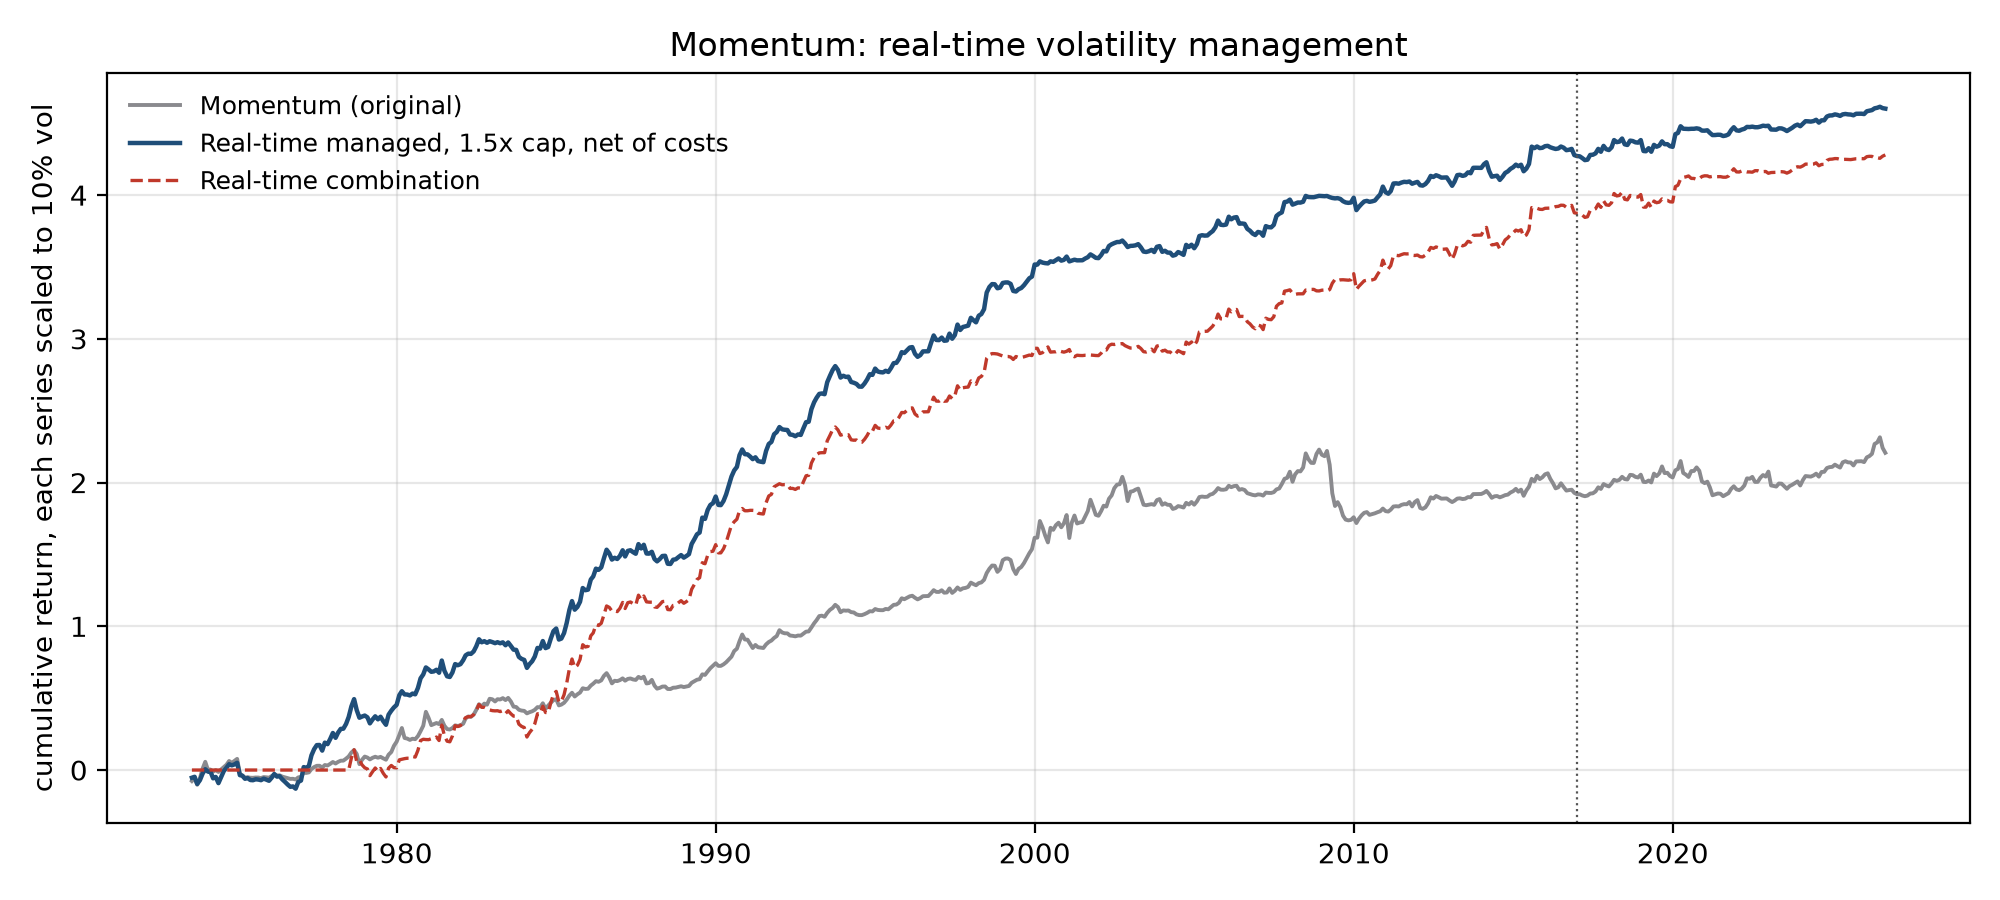
\includegraphics[width=\textwidth]{images/realtime_mom.png}
\caption{Cumulative summed monthly returns of momentum, its real-time managed version (cap 1.5, net of costs) and the real-time combination, each scaled to 10\% annualized volatility for display. Scaling leaves each Sharpe ratio unchanged. The dotted line marks January 2017, when the published samples end.}
\label{fig:mom}
\end{figure}

\section{Conclusion}

Volatility management is not a general improvement to factor investing. Built in real time with capped leverage and costs, it improves only momentum, and after the published samples even that gain is smaller and statistically uncertain. For value and investment, the same rule has cost money in the most recent decade. The deciding feature is whether a factor's returns arrive in calm or turbulent months, which an investor can check before adopting the rule.

Two limits apply. The post-2016 window has 116 months, so it can detect large differences, such as value's, but not moderate ones. We charge costs only on changes in exposure to each factor, not on the trading inside the factor portfolios, so all net figures are upper bounds.

\bigskip
\noindent\textbf{Data availability.} Factor returns are publicly available from the Kenneth R. French Data Library. Code is available from the author on request.

\noindent\textbf{Declaration of generative AI and AI-assisted technologies in the writing process.} [To be completed by the author before submission, as required by Elsevier.]

\begin{thebibliography}{10}
\bibitem[Barroso and Detzel(2021)]{barroso2021} Barroso, P., Detzel, A., 2021. Do limits to arbitrage explain the benefits of volatility-managed portfolios? \textit{Journal of Financial Economics} 140(3), 744-767.
\bibitem[Barroso and Santa-Clara(2015)]{barroso2015} Barroso, P., Santa-Clara, P., 2015. Momentum has its moments. \textit{Journal of Financial Economics} 116(1), 111-120.
\bibitem[Cederburg et al.(2020)]{cederburg2020} Cederburg, S., O'Doherty, M.S., Wang, F., Yan, X.S., 2020. On the performance of volatility-managed portfolios. \textit{Journal of Financial Economics} 138(1), 95-117.
\bibitem[Daniel and Moskowitz(2016)]{daniel2016} Daniel, K., Moskowitz, T.J., 2016. Momentum crashes. \textit{Journal of Financial Economics} 122(2), 221-247.
\bibitem[Holm(1979)]{holm1979} Holm, S., 1979. A simple sequentially rejective multiple test procedure. \textit{Scandinavian Journal of Statistics} 6(2), 65-70.
\bibitem[Ledoit and Wolf(2008)]{ledoit2008} Ledoit, O., Wolf, M., 2008. Robust performance hypothesis testing with the Sharpe ratio. \textit{Journal of Empirical Finance} 15(5), 850-859.
\bibitem[Liu et al.(2019)]{liu2019} Liu, F., Tang, X., Zhou, G., 2019. Volatility-managed portfolio: Does it really work? \textit{Journal of Portfolio Management} 46(1), 38-51.
\bibitem[McLean and Pontiff(2016)]{mclean2016} McLean, R.D., Pontiff, J., 2016. Does academic research destroy stock return predictability? \textit{Journal of Finance} 71(1), 5-32.
\bibitem[Moreira and Muir(2017)]{moreira2017} Moreira, A., Muir, T., 2017. Volatility-managed portfolios. \textit{Journal of Finance} 72(4), 1611-1644.
\end{thebibliography}

\end{document}
